\documentclass[conference, onecolumn]{IEEEtran}
\IEEEoverridecommandlockouts
% The preceding line is only needed to identify funding in the first footnote. If that is unneeded, please comment it out.

\usepackage{cite}
\usepackage{amsmath,amssymb,amsfonts}
\usepackage{algorithmic}
\usepackage{graphicx}
\usepackage{textcomp}
\usepackage{xcolor}

% \textwidth 6.5in
% \textheight 10.in

\def\BibTeX{{\rm B\kern-.05em{\sc i\kern-.025em b}\kern-.08em
    T\kern-.1667em\lower.7ex\hbox{E}\kern-.125emX}}
\begin{document}

\title{Architectural Study of Flutter\\
% {\footnotesize \textsuperscript{*}Note: Sub-titles are not captured in Xplore and
% should not be used}
% \thanks{Identify applicable funding agency here. If none, delete this.}
}

\author{\IEEEauthorblockN{VJS Pranavasri}
\IEEEauthorblockA{\textit{Interational Institute of Information Technology, Hyderabad} \\
Hyderabad, India \\
vjs.pranavasri@research.iiit.ac.in}
}

\maketitle

\begin{abstract}
This document is a paper that studies the architecture of Flutter in detail, and tries to find out any significant ideas or flaws.
\end{abstract} 

\begin{IEEEkeywords}
    flutter, android, web, cross-platform
\end{IEEEkeywords}

\section{Introduction}
Flutter is a Fluid UI framework for developing efficient mobile apps. It started as a plugin for the Flutter SDK, but it has grown into a complete framework. Google initially created Flutter as a new mobile UI framework to replace the native Android UI framework and the native iOS UI framework. The main reason for creating Flutter was to make app development easier for the developers and to create cross-platform applications. Flutter is based on Dart language and is open source and cross-platform. Flutter aimed to solve a developer or a company's trouble of having to write and maintain multiple code bases for different platforms. This is similar to what java aims at doing, "Write Once and Run Everywhere", Flutter seems to follow suit at a higher abstraction level closely. \\
In October 2011, Google unveiled Dart, with the goal of making programming web applications easier. The project was led by Lars Bak and Kasper Lund. Dart's original design was heavily influenced by JavaScript, but it also borrowed some features from other programming languages. For example, Dart supported class-based inheritance, a feature not present in JavaScript at the time. In November 2013, Google released Dart 1.0. This marked the first stable release of the language. Over the next few years, Dart gained popularity among developers as an alternative to JavaScript for web development. In 2015, Google launched the AngularDart framework, which allowed developers to build single-page web applications using Dart and AngularJS (a popular JavaScript framework). In 2016, Google released Flutter. \\ 
Before flutter came in, Android development was done in Java, Kotlin was slowly starting to replace it and iOS development was done in Objective-C, now Swift. Although flutter was revolutionary in its own right, it was not the first cross-platform mobile UI framework. React Native was one of the first cross-platform mobile UI frameworks but it lacked in many aspects. One of the major ones was native Android/iOS integration. Apps built with React Native needed an environment on which they could run javascript to simulate the app. I.e. React Native apps needed a bridge to communicate with the native code. On the other hand, flutter instead has a compilation process that converts the Dart code to native apps for respective platforms. A comparison between how flutter and react native talk to the android is shown in Figures~\ref{comparison}. \\

\begin{figure}[h]\label{comparison}
    \centering
    \begin{minipage}[b]{0.4\textwidth}
        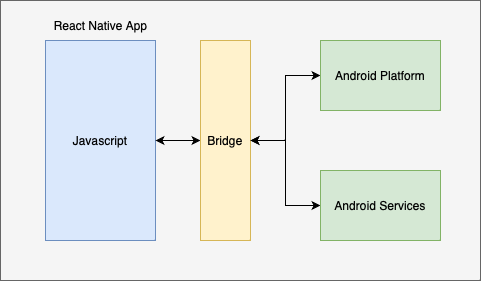
\includegraphics[width=\textwidth]{images/flutter-rn.drawio.png}
        \caption{React Native communicating with the native code}
    \end{minipage}
    \hfill
    \begin{minipage}[b]{0.4\textwidth}
        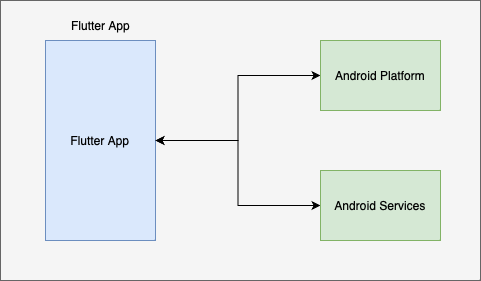
\includegraphics[width=\textwidth]{images/flutter-fl.drawio.png}
        \caption{Flutter communicating with the native code}
    \end{minipage}
\end{figure}
There are four key stakeholder groups for Flutter: developers, designers, product owners, and users.
\begin{itemize}
    \item Developers are responsible for building the app and ensuring it meets the requirements set by the product owner. They also need to be able to work with the designer to ensure that the app is visually appealing and easy to use. 
    \item Designers are responsible for creating the look and feel of the app. They need to be able to work with developers to ensure that the app is both functional and visually appealing. 
    \item Product owners are responsible for setting the direction for the app. They need to be able to work with both developers and designers to ensure that the app meets their vision. 
    \item Users are ultimately responsible for using the app. They need to be able to find value in it and use it in their everyday lives.
\end{itemize} 
These are just the top level view of the stake holders in the next section we'll broadly classify the stakeholders.

As of 2022, Flutter is the 14th most popular repository on GitHub with over 126,000 stars and supports 
the following platforms:
\begin{itemize}
\item Android (5.0 Lollipop or later)
\item iOS (9.0 or later)
\item Windows 10
\item macOS 10.15 Catalina or later
\item Linux
\item Web
\end{itemize}

\section{Relationship to the Architecture Business Cycle}
We start this section by looking at all the major stakeholder in greater detail. We follow the the classification of stakeholders by Rozanski et al. Table 1~\ref{relationship} is the brief overview of the stakeholder groups.
% Create a table of rozanski's 10 stake holders and their roles.
\begin{table}[h]
    \centering
    \label{relationship}
    \begin{tabular}{|l|l|}
        \hline
        \textbf{Stakeholder} & \textbf{Role} \\
        \hline
        \textit{Acquirers} & \textit{Oversee the procurement of the system} \\
        \hline
        \textit{Assessors} & \textit{Oversee conformance to standards and legal regulations} \\
        \hline
        \textit{Communicators} & \textit{Explain the system via documentation and training} \\
        \hline
        \textit{Developers} & \textit{Construct and deploy the system from its specifications} \\
        \hline
        \textit{Maintainers} & \textit{Manage the evolution of the system once operational} \\
        \hline
        \textit{Suppliers} & \textit{Provide hardware/software platform on which the system will run} \\
        \hline
        \textit{Support staff} & \textit{Assist users to make use of the running system} \\
        \hline
        \textit{System administrators} & \textit{Run the system once deployed} \\
        \hline
        \textit{Testers} & \textit{Check whether the system meets its specifications} \\
        \hline
        \textit{Users} & \textit{Define the system’s functionality and use it once running} \\
        \hline
    \end{tabular} \\
    \caption{Rozanski Wood's classification of the stakeholders\cite{ssa}}
    \label{relationship}
\end{table}
\textbf{Acquirers} - This is probably the easiest to answer and guess. Google is the acquirer of flutter, and the whole flutter team works under google. \\
\textbf{Assessors} - Although this is one of the most major parts, there is no particular entity overseeing the conformance to standards, as the project is open sourced under BSD Lisencse\cite{3ClauseBSDLicense}, this makes it free for any individual or company to contribute or use. Even then any change has to at least be reviewed by two core memebers before being merged into code, which could make them the Assessors. \\
\textbf{Communicators} - Most of the communication regarding the code, how to use it, and any new updates happen completely through their official websites, launch events and documentation. \\
\textbf{Developers and Maintainers} - The developers and maintainers are the main contributors to the project. They are the ones who write the code and the ones who maintain the code. Currently, there are 91 Developers to the flutter codebase, all of whom are mentioned in their github repo. \\
\textbf{Suppliers} - This would the same as Users, as this would run on the system of whoever is using flutter. \\
\textbf{Support} - The majority of the support is provided by google support, and other major forms would be through stackoverflow and their documentation. \\
\textbf{Testers} - For testing the code, a lot of automated test cases are written in every iteration at both the level of flutter and dart to make sure everything that's added and everything that already exists works well. \\
\textbf{Users} - The users are all the open source developers, private developers and companies who may use flutter however they like. \\

For looking at how the architect's decision might have been made, we look at the architecture business cycle, rather a very particular diagram that shows the power vs interest of different stakeholders. We use this diagram\ref{architecture} to try to understand the architectural decisions made by the team.
\begin{figure}[h]\label{architecture}
    \centering 
    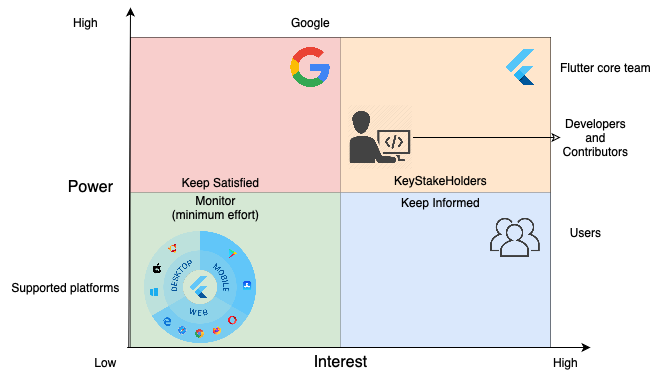
\includegraphics[width=\textwidth]{images/flutter-pow-int.drawio.png}
    \caption{Power vs Interest Graph}
\end{figure}
Obviously, from the figure, we can see that the core flutter team has the most power and most interest in the project, so this would make the job of the architect a bit easier as this might usually not be the case. The next entity holding the highest power is Google. Google would have as much power over flutter as the core team does, as it is owned by Google. The figure depicts a relative interest comparison and in no way suggests that the given stakeholder(Google) would be less interested in the project. It just signifies that Flutter team has the highest interest, and although google might have great interest in the project it would not be as much as flutter core team. Therefore we put it very close to the border signifying the interest part. But the tech lead(Ian) claims that their contributors are as much part of the flutter team as the core team is, hence we put contributors in the key stakeholders, as they have a bit of power and interest both on the higher side than normal. 
Next come the users, who have the highest amount of interest, and their power comes from the ability to give feedback. And lastly the systems Flutter sdk is built in and built for, these are all minimum effort to look after and do not posses such high power or interest.

\section{Requirements and Qualities}
\color{blue}
What were the key functional requirements? What were the key quality attributes that the system had to exhibit? Why? What was the relative ranking of these attributes? Why? If feasible, give examples of how the quality attributes are visible in the delivered.
\color{black}

\section{Architectural Solution}
\color{blue}
This section is the most important part of the report, and should clearly describe the architecture and how it achieved (or failed to achieve) its functional and quality goals.
What are the key aspects of resulting architecture? What views are most appropriate for illustrating the architects' approach to achieving the functional and quality requirements? What is the content of these views (graphics should appropriately be provided here). Be sure to include a discussion of any alternatives considered and/or the rationale for the architectural choices made. Identify specific patterns and/or tactics found in the architecture.
\color{black}

\section{Summary}
\color{blue}
Briefly reflect on the system you researched. Did it meet its goals? Is it exemplary in some respects? What are its strengths and weaknesses relative to the desired functionality and qualities? Is there anything of note about the system that is not described in one of the previous sections?
\color{black}

% \section{References} taken care of by the bibliography
\bibliographystyle{IEEEtran}
\bibliography{references}

\appendix
Just in case I want to add an appendix

\section*{Effort}
VJS Pranavasri : X hours

\vspace{12pt}
\color{red}
This is just the format for the report. The actual report is yet to be added.

\end{document}
